\documentclass[12pt,a4paper]{article}
\synctex=1
\usepackage[utf8]{inputenc}
\usepackage[margin=1cm,bottom=2cm]{geometry}
\usepackage{graphicx}
%\usepackage{verbatim}
\usepackage{listings}
\usepackage{multicol}
\usepackage{libertine}
\usepackage{pgfornament}
\usepackage{eso-pic}
\usepackage{textcomp}
\usepackage{courier}
\usepackage[hangul]{kotex}
\linespread{1.3}

\title{
	\centering
	\pgfornament[width=12cm,color=teal]{84}\\
	\vspace{1cm}
	\fontsize{50}{50} \selectfont {시스템 S/W 실습11}\\
	\pgfornament[width=12cm,color=teal]{88}\\
	\vfill}
\author{
	\LARGE
	\begin{tabular}{rl}
		\hline
		학번 : & 2016110056\\ 
		학과 : & 불교학부 \\
		이름 : & 박승원\\
		날짜 : & \today\\
		\hline
	\end{tabular}\vspace{2cm}
	\\
	\includegraphics[width=0.5\textwidth]{/home/zezeon/Dropbox/Photos/logo.jpg}
}
\date{}


\begin{document}
\maketitle
\newpage
\noindent
\lstset{columns=flexible, tabsize=4, frame=single, showstringspaces=false, breaklines=true, upquote=true}

\pagenumbering{gobble}
\lstset{language=C}
%\begin{multicols}{2}
\begin{enumerate}
\item 파일 처리

\lstinputlisting[caption=file.c]{file.c}

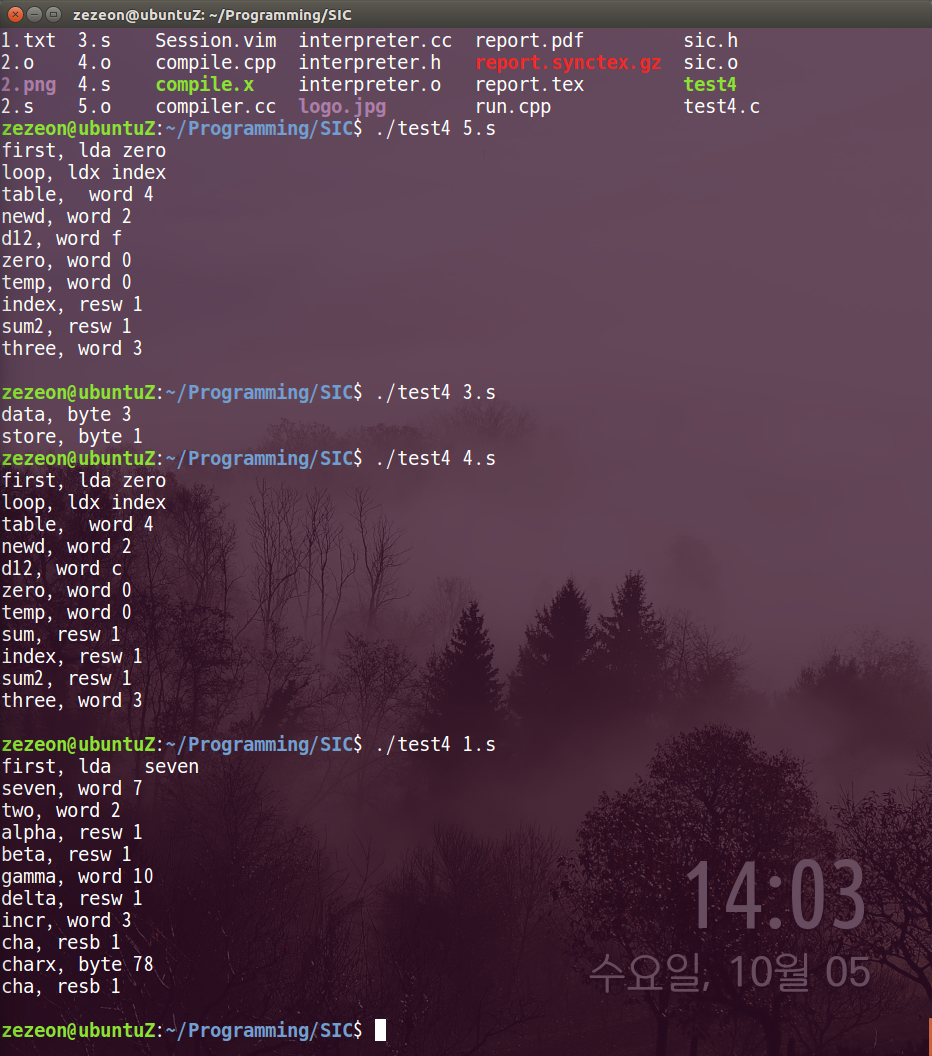
\includegraphics[width=\textwidth]{1.png}

\item 다음에 주어진 MacroAssembly program MacroSrcfile.txt file을 읽어서 각 줄을 LABEL, OPCODE, OPERAND로 분리하여 Intfile에 출력하면서 Macro Definition Table MDT[]와 macro Name Table MNT[]를 생성하고, MDT[]와 MNT[]의 내용을 출력하는 Macro Processor PASS1에 해당하는 프로그램 MacroPass1를 구현하고 실습하시오.
단, C Program compile명령은 다음과 같고, 입력파일 MacroSrcfile.txt file은 e-class에서 download 할 수 있다.

\$gcc -o MacroPass1 MacroPass1.c

\$./MacroPass1 MacroSrcfile.txt

\lstinputlisting[caption=MacroPass1.c]{pass2.cpp}

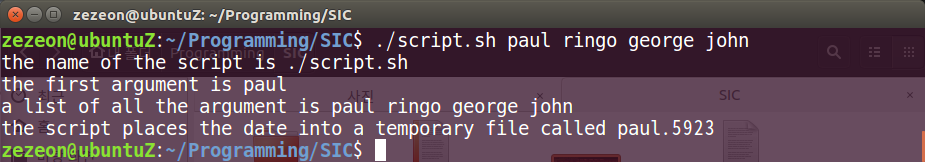
\includegraphics[width=0.9\textwidth]{2.png}
실행시 매크로 부분만 따로 출력해준다.

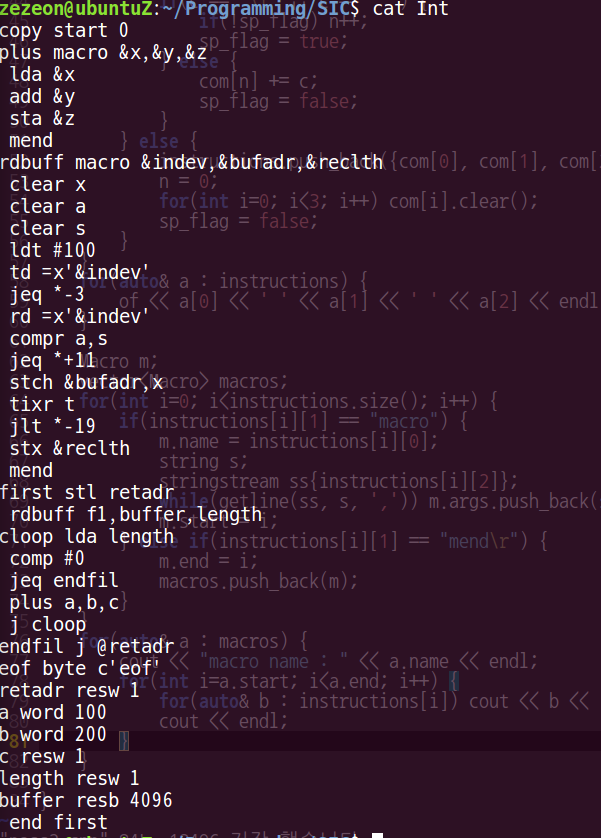
\includegraphics[width=0.7\textwidth]{3.png}
인스트럭션을 구분한 Int파일의 내용을 출력해보았다.
\end{enumerate}
{\Huge소감}
\indent
write(fd, "/0", 1)에서 한글자만 쓰기 때문에 /////로 나오는 것이었다. 항상 교수님께서 퀴즈를 하나씩 내주시는 것 같다.
개행문자가 유닉스와 윈도우즈간에 호환이 안 되어 소스 파일을 처리하는 데에 애를 먹었다.

\end{document}
